\documentclass[a4paper, 11pt]{article}
\usepackage{graphicx}
\usepackage{multicol}
\usepackage{tabularx}
\usepackage{enumitem}
\usepackage[a4paper, margin=1.8cm]{geometry}
\usepackage{listings}
\usepackage{amssymb}
\usepackage{gvv}
\usepackage{gvv-book}
\usepackage{amsmath}
\usepackage{setspace}
\usepackage{caption}

\graphicspath{ {./figs/} }

\begin{document}

\begin{center}
    \huge{CS: COMPUTER SCIENCE AND INFORMATION TECHNOLOGY}\\
    \large{EE25BTECH11041 - Naman}
\end{center}

\begin{enumerate}
    \item Which of the following is NOT necessarily a property of a Group?
    \begin{enumerate}
    \begin{multicols}{2}
    \item Associativity
    \item Commutativity
    \item Existence of inverse for every element
    \item Existence of identity
    \end{multicols}
    \end{enumerate}
    

    \hfill (GATE CS 2009)
    
    \item What is the chromatic number of an n-vertex simple connected undirected graph which does not contain any odd lenght cycle? Assume $n \geq 2$
    \begin{enumerate}
        \begin{multicols}{4}
            \item 2
            \item 3
            \item 4
            \item 5
        \end{multicols}
    \end{enumerate}

    \hfill (GATE CS 2009)

    \item Which one of the following is TRUE for any simple connected undirected graph with more than 2 vertices?
    \begin{enumerate}
        \item No two vertices have the same degree.
        \item At least two vertices have the same degree.
        \item At least three vertices have the same degree.
        \item All vertices have the same degree.
    \end{enumerate}

    \hfill (GATE CS 2009)

    \item Consider the binary relation $R = {(x, y), (x, z), (z, x), (z, y)}$ on the set ${x, y, z}$. Which one of the following is TRUE?
    \begin{enumerate}
        \begin{multicols}{2}
            \item R is symmetric but NOT antisymmetric.
            \item R is NOT symmetric but antisymmetric.
            \item R is both symmetric and antisymmetric.
            \item R is neither symmetric nor antisymmetric.
        \end{multicols}
    \end{enumerate}

    \hfill (GATE CS 2009)

    \item $(1217)_8$ is equivalent to
    \begin{enumerate}
        \begin{multicols}{4}
            \item $(1217)_{16}$
            \item $(028F)_{16}$
            \item $(2297)_{10}$
            \item $(0B17)_{16}$
        \end{multicols}
    \end{enumerate}

    \hfill (GATE CS 2009)

    \item What is the minimum number of gates required to implement the Boolean function $(AB + C)$ if we have to use only 2-input NOR gates?
    \begin{enumerate}
        \begin{multicols}{4}
            \item 2
            \item 3
            \item 4
            \item 5
        \end{multicols}
    \end{enumerate}

    \hfill (GATE CS 2009)

    \item How many $32K \times 1 RAM$ chips are needed to provide a memory capacity of 256 K-bytes?\\
    \begin{enumerate}
        \begin{multicols}{4}
            \item 8
            \item 32
            \item 64
            \item 128
        \end{multicols}
    \end{enumerate}

    \hfill (GATE CS 2009)

    \item A CPU generally handles an interrupt by executing an interrupt service routine
    \begin{enumerate}
        \item as soon as an interrupt is raised.
        \item by checking the interrupt register at the end of fetch cycle.
        \item by checking the interrupt register after finishing the execution of the current instruction.
        \item by checking the interrupt register at fixed time intervals.
    \end{enumerate}

    \item In which one of the following page replacement policies, Belady's anomaly may occur?
    \begin{enumerate}
        \begin{multicols}{4}
            \item FIFO
            \item OPTIMAL
            \item LRU
            \item MRU
        \end{multicols}
    \end{enumerate}

    \hfill (GATE CS 2009)

    \item The essential content(s) in each entry of a page table is/are
    \begin{enumerate} 
        \item virtual page number.
        \item page frame number.
        \item both virtual page number and page frame number.
        \item access right information.
    \end{enumerate}

    \hfill (GATE CS 2009)

    \item What is the number of swaps required to sort n elements using selection sort, in the worst case?
    \begin{enumerate}
        \begin{multicols}{4}
            \item $\Theta \textit{(n)}$
            \item $\Theta$ \textit{(n $\log n $)}
            \item $\Theta (n^2)$
            \item $\Theta$ \textit{($n^2 \log n$)}
        \end{multicols}
    \end{enumerate}

    \hfill (GATE CS 2009)

    \item $S \rightarrow aSa | bSb| a | b$\\The language generated by the above grammar over the alphabet ${a, b}$ is the set of
    \begin{enumerate} 
        \item all palindromes.
        \item all odd length palindromes.
        \item strings that begin and end with the same symbol.
        \item all even length palindromes.
    \end{enumerate}

    \hfill (GATE CS 2009)

    \item Which of the following statement(s) is/are correct regarding Bellman-Ford shortest path algorithm?
    \begin{enumerate}[label= \Alph*, start=16]
        \item Always finds a negative weighted cycle, if one exists.
        \item Finds whether any negative weighted cycle is reachable from the source.
    \end{enumerate}
    \begin{enumerate} 
        \item P only
        \item Q only
        \item Both P and Q
        \item neither P and Q
    \end{enumerate}

    \hfill (GATE CS 2009)

    \item Let $\pi_A$ be a problem that belongs to the class NP. Then which one of the following is TRUE?
    \begin{enumerate}
        \item There is no polynomial time algorithm for $\pi_A$.
        \item If $\pi_A$, can be solved deterministically in polynomial time, then P = NP.
        \item If $\pi_A$ is NP-hard, then it is NP-complete.
        \item $\pi_A$ may be undecidable.
    \end{enumerate}

    \hfill (GATE CS 2009)

    \item Which one of the following languages over the alphabet $(0, 1)$ is described by the regular expression: $(0+1)*0(0+1)*0(0+1)*$?
    \begin{enumerate} 
        \item The set of all strings containing the substring 00. 
        \item The set of all strings containing at most two 0's.
        \item The set of all strings containing at least two 0's.
        \item The set of all strings that begin and end with either 0 or 1.
    \end{enumerate}

    \hfill (GATE CS 2009)

    \item Which one of the following is FALSE?
    \begin{enumerate} 
        \item There is a unique minimal DFA for every regular language.
        \item Every NFA can be converted to an equivalent PDA.
        \item Complement of every context-free language is recursive.
        \item Every nondeterministic PDA can be converted to an equivalent deterministic PDA.
    \end{enumerate}

    \hfill (GATE CS 2009)

    \item Match all items in Group 1 with correct options from those given in Group 2.\\
    \begin{tabular}{ll}
        Group 1 & Group 2 \\
        P. Regular expression & 1. Syntax analysis\\
        Q. Pushdown automata & 2. Code generation\\
        R. Dataflow analysis & 3. Lexical analysis \\
        S. Register allocation & 4. Code Optimization
    \end{tabular}
    
    \begin{enumerate} 
        \item P-4, Q-1, R-2, S-3
        \item P-3, Q-1, R-4, S-2 
        \item P-3, Q-4, R-1, S-2
        \item P-2, Q-1, R-4, S-3
    \end{enumerate}

    \hfill (GATE CS 2009)

    \item Consider the program below:
    \begin{lstlisting}
    #include <stdio.h>
    int fun(int n, int *f_p) {
        int t, f;
        if (n <= 1) {
        *f_p + 1:
        return 1:
        }
        t = fun (n-1, f_p);
        f = t + *f_p;
        return f;
    }
    int main(){
        int x = 15;
        printf("%d\n", fun(5, &x));
        return 0;
    }
    \end{lstlisting}
    The value printed is: 
    \begin{enumerate}
        \begin{multicols}{4}
            \item 6
            \item 8
            \item 14
            \item 15
        \end{multicols}
    \end{enumerate}

    \hfill (GATE CS 2009)

    \item The coupling between different modules of a software is categorized as follows:
    \begin{enumerate}[label=\Roman*]
        \item Content coupling
        \item Common coupling 
        \item Control coupling
        \item Stamp coupling
    \end{enumerate}
    Coupling between modules can be ranked in the order of strongest (least desirable) to weakest (most desirable) as follows:
    \begin{enumerate}
        \begin{multicols}{2}
            \item I-II-III-IV-V 
            \item V-IV-III-II-I
            \item I-III-VII-IV
            \item IV-II-V-III-I
        \end{multicols}
    \end{enumerate}

    \hfill (GATE CS 2009)

    \item Consider the HTML table definition given below:
    \begin{lstlisting}
    <table border=1>
        <tr> <td rowspan=2> ab </td>
        <td colspan=2> cd </td>
        </tr>
        <tr> <td> ef </td>
        <td rowspan=2> gh </td>
        </tr>
        <tr> <td colspan=2> ik </td>
        </tr>
    </table>
    \end{lstlisting}
    The number of rows in each column and the number of columns in each row are: 
    \begin{enumerate}
        \begin{multicols}{2}
            \item (2,2,3) and (2,3,2)
            \item (2,3,2) and (2,3,2)
            \item (2,2,3) and (2,2,3)
            \item (2,3,2) and (2,2,3)
        \end{multicols}
    \end{enumerate}

    \hfill (GATE CS 2009)

    \item An unbalanced dice (with 6 faces, numbered from 1 to 6) is thrown. The probability that the face value is odd is $90\%$ of the probability that the face value is even. The probability of getting any even numbered face is the same.\\
    If the probability that the face is even given that it is greater than 3 is 0.75, which one of the following options is closest to the probability that the face value exceeds 3?
    \begin{enumerate}
        \begin{multicols}{4}
            \item 0.453
            \item 0.468
            \item 0.485
            \item 0.492
        \end{multicols}
    \end{enumerate}


    \hfill (GATE CS 2009)

    \item  For the composition table of a cyclic group shown below\\
    \begin{tabular}{c|cccc}
        * &a &b &c &d \\
        \hline
        a &a &b &c &d \\
        b &b &a &d &a \\
        c &c &d &b &b \\
        d &d &c &a &c \\
        
    \end{tabular}\\
    Which one of the following choices is correct?
    \begin{enumerate}
        \begin{multicols}{2}
            \item $a, b$ are generators
            \item $c, d$ are generators
            \item $b, c$ are generators
            \item $d, a$ are generators
        \end{multicols}
    \end{enumerate}

    \hfill (GATE CS 2009)

    \item Which one of the following is the most appropriate logical formula to represent the statement:
    \begin{center}
        \textit{"Gold and silver ornaments are precious"}
    \end{center}
    The following notations are used:

        \begin{itemize}
            \item $G(x): x$ is a gold ornament.
            \item $S(x): x$ is a silver ornament.
            \item $P(x): x$ is precious.
        \end{itemize}

    \begin{enumerate}
        \begin{multicols}{2}
            \item $\forall x(P(x)\rightarrow (G(X)\land S(x)))$
            \item $\forall x((G(X)\land S(x)))\rightarrow P(x)$
            \item $\exists x((G(X)\land S(x)))\rightarrow P(x)$
            \item $\forall x(P(x)\rightarrow (G(X)\lor S(x)))$
        \end{multicols}
    \end{enumerate}

    \hfill (GATE CS 2009)

    \item  The binary operation is defined as follows:\\
    \begin{tabular}{|c|c|c|}
        \hline
        P & Q & $P\square Q$ \\
        \hline
        T & T & T \\
        \hline
        T & F & T \\
        \hline
        F & T & F \\
        \hline
        F & F & T\\
        \hline
    \end{tabular}\\
    Which one of the following is equivalent to $P \lor Q$?
    \begin{enumerate}
        \begin{multicols}{2}
            \item $\neg_ Q \square \neg_ P$
            \item $ P \square \neg_Q $
            \item $ \neg_ P \square Q $
            \item $\neg_ P \square \neg_ Q$
        \end{multicols}
    \end{enumerate}

    \item $\int_0^{\pi/4} (1 - \tan x)(1 + \tan x)dx$\\
    evalutes to
    \begin{enumerate}
        \begin{multicols}{2}
            \item 0
            \item 1
            \item $\ln2$
            \item $1/2\ln2$
        \end{multicols}
    \end{enumerate}

    \hfill (GATE CS 2009)

    \item Consider the following well-formed formulae:\\
    \begin{enumerate}[label=\Roman*]
        \item $\neg_ \forall (P(x))x$
        \item $\neg_ \exists (P(x))x$
        \item $\neg_ \exists (\neg_ P(x))x$
        \item $\forall (\neg_ P(x))x$
    \end{enumerate}

    Which of the above are equivalent ?

    \begin{enumerate}
        \begin{multicols}{2}
            \item I and III 
            \item I and IV
            \item II and III
            \item II and IV
        \end{multicols}
    \end{enumerate}

    \hfill (GATE CS 2009)

    \item Given the following state table of an FSM with two states A and B, one input and one output:\\
    \begin{tabular}{|c|c|c|c|c|c|}
    \hline
        Present State A  & Present State B  & Input & New State A & New State B & Output\\
        \hline
        0  & 0  & 0 & 0 & 0 & 1\\
        \hline
        0  & 1  & 0 & 1 & 0 & 0\\
        \hline
        1  & 0  & 0 & 0 & 1 & 0\\
        \hline
        1  & 1  & 0 & 1 & 0 & 0\\
        \hline
        0  & 0  & 1 & 0 & 1 & 0\\
        \hline
        0  & 1  & 1 & 0 & 0 & 1\\
        \hline
        1  & 0  & 1 & 0 & 1 & 1\\
        \hline
        1  & 1  & 1 & 0 & 0 & 1\\
        \hline
    \end{tabular}

        If the initial state is $A = 0, B = 0$, what is the minimum length of an input string which will take the machine to the state $A= 0, B = 1$ with Output = 1?
        \begin{enumerate}
        \begin{multicols}{4}
            \item 3
            \item 4
            \item 5
            \item 6
        \end{multicols}
        \end{enumerate}

        \hfill (GATE CS 2009)

    \item Consider a 4 stage pipeline processor. The number of cycles needed by the four instructions 11, 12, 13, 14 in stages $S1, S2, S3, S4$ is shown below:\\
    \begin{center}
        \begin{tabular}{|c|c|c|c|c|}
    \hline
           & S1  & S2 & S3 & S4 \\
        \hline
        11  & 2  & 1 & 1 & 1 \\
        \hline
        12  & 1  & 3 & 2 & 2 \\
        \hline
        13  & 2  & 1 & 1 & 3 \\
        \hline
        14  & 1  & 2 & 2 & 2 \\
        \hline
    \end{tabular}
    \end{center}
    

    What is the number of cycles needed to execute the following loop?\\
        \begin{center}
            for(i=1 to 2) (11;12;13;14;)\\
        \end{center}
        \begin{enumerate}
        \begin{multicols}{4}
            \item 16
            \item 23
            \item 28
            \item 30
        \end{multicols}
        \end{enumerate}

    \hfill (GATE CS 2009)

    \item Consider a 4-way set associative cache (initially empty) with total 16 cache blocks. The main memory consists of 256 blocks and the request for memory blocks is in the following order:
    
    \begin{center}
        0, 255, 1, 4, 3, 8, 133, 159, 216, 129, 63, 8, 48, 32, 73, 92, 155.\\
    \end{center}
    
    Which one of the following memory block will NOT be in cache if LRU replacement policy is used?
        \begin{enumerate}
        \begin{multicols}{4}
            \item 3
            \item 8
            \item 129
            \item 216
        \end{multicols}
        \end{enumerate}

    \hfill (GATE CS 2009)

    \item Consider a system with 4 types of resources $R1 (3 units), R2 (2 units), R3 (3 units), R4 (2 units)$. A non-preemptive resource allocation policy is used. At any given instance, a request is not entertained if it cannot be completely satisfied. Three processes P1, P2, P3 request the resources as follows if executed independently.\\
    \begin{tabular}{|l|l|l|}
    \hline
        Process P1: & Process P2: & Process P3: \\
        t=0: requests 2 units of R2 & t=0: requests 2 units of R3 & t = 0: requests 1 unit of R4 \\
        t=1: requests 1 unit of R3 & t=2: requests 1 unit of R4 & t=2: requests 2 units of RI \\
        t=3: requests 2 units of R1 & t=4: requests 1 unit of R1 & t = 5: releases 2 units of R1 \\
        t=5: releases 1 unit of R2 and\\ 1 unit of R1 & t = 6: releases 1 unit of R3 & t=7: requests 1 unit of R2 \\
        t=7: releases 1 unit of R3 & t = 8: Finishes & t = 8: requests 1 unit of R3 \\
        t = 8: requests 2 units of R4 &  &  t=9: Finishes \\
        t=10: Finishes &  & \\
        \hline
    \end{tabular}

    Which one of the following statements is TRUE if all three processes run concurrently starting at time t=0?
    \begin{enumerate} 
        \item All processes will finish without any deadlock.
        \item Only P1 and P2 will be in deadlock.
        \item Only P1 and P3 will be in deadlock.
        \item All three processes will be in deadlock.
    \end{enumerate}

    \hfill (GATE CS 2009)

    \item Consider a disk system with 100 cylinders. The requests to access the cylinders occur in following sequence:
    \begin{center}
        4, 34, 10, 7, 19, 73, 2, 15, 6, 20.
    \end{center}
    Assuming that the head is currently at cylinder 50, what is the time taken to satisfy all requests if it takes 1 ms to move from one cylinder to adjacent one and shortest seek time first policy is used?\\
    \begin{enumerate}
        \begin{multicols}{4}
            \item 95 ms
            \item 119 ms
            \item 233 ms
            \item 276 ms
        \end{multicols}
    \end{enumerate}

    \hfill (GATE CS 2009)

    \item In the following process state transition diagram for a uniprocessor system, assume that there are always some processes in the ready state:\\
    \begin{figure}[H]
        \centering
        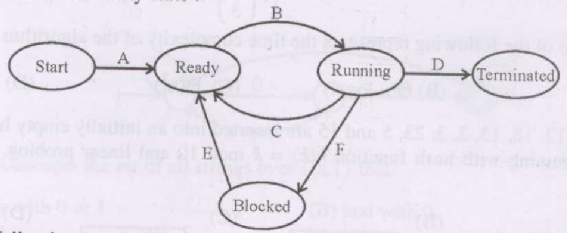
\includegraphics[width=\columnwidth]{figs/q32.png}
        \caption{}
        \label{fig:placeholder}
    \end{figure}

    Now consider the following statements:

    \begin{enumerate}[label=\Roman*]
        \item If a process makes a transition D, it would result in another process making transition A immediately.
        \item A process P2 in blocked state can make transition E while another process P, is in running state.
        \item The OS uses preemptive scheduling.
        \item The OS uses non-preemptive scheduling.
    \end{enumerate}
    Which of the above statements are TRUE?\\

    \begin{enumerate}
        \begin{multicols}{4}
            \item I and II
            \item I and III
            \item II and III
            \item II and IV
        \end{multicols}
    \end{enumerate}

    \hfill (GATE CS 2009)

    \item he enter \verb|_CS ()| and leave \verb|_CS()| functions to implement critical section of a process are realized using test-and-set instruction as follows:\\
    \begin{lstlisting}
        void enter_CS(X)
        {
            while (test-and-set(X));
            
        }

        void leave_CS(X){
         X=0;
        }
        
    \end{lstlisting}
    In the above solution, X is a memory location associated with the CS and is initialized to 0. Now consider the following statements:\\
    I. The above solution to CS problem is deadlock-free.\\
    II. The solution is starvation free.\\
    III. The processes enter CS in FIFO order.\\
    IV. More than one process can enter CS at the same time.\\
    Which of the above statements are TRUE?\\
    \begin{enumerate}
        \begin{multicols}{4}
            \item I only
            \item I and II
            \item II and III
            \item IV only
        \end{multicols}
    \end{enumerate}

    \hfill (GATE CS 2009)
    
    \item A multilevel page table is preferred in comparison to a single level page table for translating virtual address to physical address because
    \begin{enumerate} 
        \item  it reduces the memory access time to read or write a memory location.
        \item it helps to reduce the size of page table needed to implement the virtual address space of a process. 
        \item it is required by the translation lookaside buffer.
        \item it helps to reduce the number of page faults in page replacement algorithms.
    \end{enumerate}

    \hfill (GATE CS 2009)

    \item The running time of an algorithm is represented by the following recurrence relation :\\
    \begin{align}
        T(n) &=
    \begin{cases}
        n, & n \leq 3,\\
        T\!\left(\frac{n}{3}\right) + cn, & \text{otherwise}.
    \end{cases}
    \end{align}

    Which one of the following represents the time complexity of the algorithm?
    \begin{enumerate}
        \begin{multicols}{4}
            \item $\Theta(n) $
            \item $\Theta(n \log n)$
            \item $\Theta(n^2)$
            \item $\Theta(n^2 \log n)$
        \end{multicols}
    \end{enumerate}

    \hfill (GATE CS 2009)

    \item  The keys $12, 18, 13, 2, 3, 23, 5 and 15$ are inserted into an initially empty hash table of length 10 using open addressing with hash function h(k) = k mod 10 and linear probing. What is the resultant hash table?
    \begin{enumerate}
        \begin{multicols}{4}
        
            \item \begin{tabular}{|c|c|}
            \hline
            0 &  \\
            \hline
            1 &   \\
            \hline
            2 & 2 \\
            \hline
            3 & 23\\
            \hline
            4 &   \\
            \hline
            5 & 15\\
            \hline
            6 &   \\
            \hline
            7 &   \\
            \hline
            8 & 18\\
            \hline
            9 &   \\
            \hline
            \end{tabular}

        \item  \begin{tabular}{|c|c|}
            \hline
            0 &  \\
            \hline
            1 &   \\
            \hline
            2 & 2 \\
            \hline
            3 & 23\\
            \hline
            4 &   \\
            \hline
            5 & 15\\
            \hline
            6 &   \\
            \hline
            7 &   \\
            \hline
            8 & 18\\
            \hline
            9 &   \\
            \hline
            \end{tabular} 

        \item \begin{tabular}{|c|c|}
            \hline
            0 &  \\
            \hline
            1 &   \\
            \hline
            2 & 2 \\
            \hline
            3 & 23\\
            \hline
            4 &   \\
            \hline
            5 & 15\\
            \hline
            6 &   \\
            \hline
            7 &   \\
            \hline
            8 & 18\\
            \hline
            9 &   \\
            \hline
            \end{tabular} 

        \item \begin{tabular}{|c|c|}
            \hline
            0 &  \\
            \hline
            1 &   \\
            \hline
            2 & 2 \\
            \hline
            3 & 23\\
            \hline
            4 &   \\
            \hline
            5 & 15\\
            \hline
            6 &   \\
            \hline
            7 &   \\
            \hline
            8 & 18\\
            \hline
            9 &   \\
            \hline
            \end{tabular}
        
        \end{multicols}    
    \end{enumerate}

    \hfill (GATE CS 2009)

    \item What is the maximum height of any AVL-tree with 7 nodes? Assume that the height of a tree with a single node is 0.
    \begin{enumerate}
        \begin{multicols}{4}
            \item 2
            \item 3
            \item 4
            \item 5
        \end{multicols}
    \end{enumerate}


    \hfill (GATE CS 2009)

    \item Consider the following graph:

    \begin{figure}[H]
        \centering
        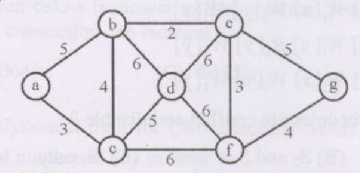
\includegraphics[width=\columnwidth]{figs/q38.png}
        \caption{}
        \label{fig:placeholder}
    \end{figure}
    Which one of the following is NOT the sequence of edges added to the minimum spanning tree using Kruskal's algorithm? 
    \begin{enumerate}
        \begin{multicols}{2}
            \item (b. e) (e, f) (a, c) (b, c) (f, g) (c, d)
            \item (b. e) (e, f) (a, c) (f. g) (b, c) (c, d)
            \item (b, e) (a, c) (e, f) (b, c) (f, g) (c, d)
            \item (b, e) (e, f) (b, c) (a, c) (f, g) (c, d)
        \end{multicols}
    \end{enumerate}

    \hfill (GATE CS 2009)

    \item In quick sort, for sorting n elements, the $(n/4)$ smallest element is selected as pivot using an $O(n)$ time algorithm. What is the worst case time complexity of the quick sort?
    \begin{enumerate}
        \begin{multicols}{4}
            \item $\Theta(n)$
            \item $\Theta(n \log n)$
            \item $\Theta(n^2)$
            \item $\Theta(n^2 \log n)$  \\
        \end{multicols}
    \end{enumerate}

    \hfill (GATE CS 2009)

    \item  Let L= $L1\bigcap L2$, where L1 and L2 are languages as defined below:
    L1 = {$a^m b^m c a^n b^n | m,n \geq0$}\\
    L2 = {$a^i b^j c^k| i,j,k \geq0$}\\
    Then L is:\\

    \begin{enumerate}
        \begin{multicols}{2}
            \item not recursive.
            \item regular 
            \item context-free but not regular.
            \item recursively enumerable but not context-free.
        \end{multicols}
    \end{enumerate}

    \hfill (GATE CS 2009)
    
    \item The above DFA accepts the set of all strings over (0, 1) that
    \begin{figure}[H]
        \centering
        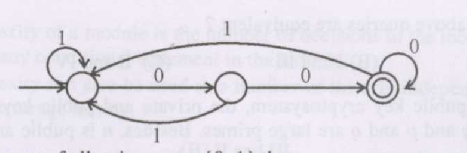
\includegraphics[width=\columnwidth]{figs/q41.png}
        \caption{}
        \label{fig:placeholder}
    \end{figure}
        
    
    \begin{enumerate}
        \begin{multicols}{2}
            \item begin either with 0 or 1.
            \item end with 0.
            \item end with 00.
            \item contain the substring 00.
        \end{multicols}
    \end{enumerate}

    \hfill (GATE CS 2009)
    
    \item Which of the following statements are TRUE?\\

    \begin{enumerate}[label=\Roman*]
        \item There exist parsing algorithms for some programming languages whose complexities are less than $O(n^3)$.
        \item A programming language which allows recursion can be implemented with static storage allocation.
        \item No L-attributed definition can be evaluated in the framework of bottom-up parsing.
        \item Code improving transformations can be performed at both source language and intermediate code level.
    \end{enumerate}
    \begin{enumerate}
        \begin{multicols}{4}
            \item I and II
            \item I and IV 
            \item II and IV
            \item I,III and IV
        \end{multicols}
    \end{enumerate}

    \hfill (GATE CS 2009)

    \item Consider two transactions T, and T2, and four schedules S1, S2, S3, S4 of T, and T2 as given below: T: \\
    $
    T_1: R_1[x] W_1[x] W_1[y]\\
    T_2: R_2[x] R_2[y] W_2[y]\\
    S_1: R_1[x] R_2[x] R_2[y] W_1[x] W_1[y] W_2[y] \\
    S_2: R_1[x] R_2[x] R_2[y] W_1[x] W_2[y] W_1[y]\\
    S_3: R_1[x] W_1[x] R_2[x] W_1[y] R_2[y] W_2[y]\\
    S_4: R_2[x] R_2[y] R_1[x] W_1[x] W_1[y] W_2[y]\\
    $
    Which of the above schedules are conflict-serializable?
    \begin{enumerate}
        \begin{multicols}{4}
            \item $S_1 and S_2$
            \item $S_2 and S_3$
            \item $S_3 only $
            \item $S_4 only$
        \end{multicols}
    \end{enumerate}

    \hfill (GATE CS 2009)

    \item The following key values are inserted into a B+-tree in which order of the internal nodes is 3, and that of the leaf nodes is 2, in the sequence given below. The order of internal nodes is the maximum number of tree pointers in each node, and the order of leaf nodes is the maximum number of data items that can be stored in it. The B+-tree is initially empty.\\
    $10, 3, 6, 8, 4, 2, 1$\\
    The maximum number of times leaf nodes would get split up as a result of these insertions is
    \begin{enumerate}
        \begin{multicols}{4}
            \item 2
            \item 3
            \item 4
            \item 5
        \end{multicols}
    \end{enumerate}

    \hfill (GATE CS 2009)

    \item Let $R and S$ be relational schemes such that $R= {a,b,c} and S = {c}$. Now consider the following queries on the database:\\
    \begin{enumerate}[label=\Roman*]
        \item $\pi_{R-S}(r)-\pi_{R-S}(\pi_{R-S}(r)\times s-\pi_{R-S,S}(r))$
        \item ${t|t \in \pi_{R-S}(r) \land \forall u \in s(\exists v \in r(u=v[s] \land t=v[R-S]))}$
        \item ${t|t \in \pi_{R-S}(r) \land \forall u \in s(\exists v \in s(u=v[r] \land t=v[R-S]))}$
        \item Select $R.a, R.b$\\ from $R, S$\\where $R.c=S.c$
    \end{enumerate}

    Which of the above queries are equivalent ?
    \begin{enumerate}
        \begin{multicols}{4}
            \item $I and II$
            \item $I and III$
            \item $II and IV$
            \item $III and IV $
        \end{multicols}
    \end{enumerate}

    \hfill (GATE CS 2009)

    \item In the RSA public key cryptosystem, the private and public keys are $(e, n) and (d, n)$respectively, where $n=p\star q and p and q$ are large primes. Besides, n is public and p and q are private. Let M be an integer such that $0<M<n$ and $o(n)=(p-1)(q-1)$. Now consider the following equations.\\
    \begin{enumerate}[label=\Roman*]
        \item $M' = M^e$  mod n\\ $M = (M')^d$ mod n
        \item $ed \equiv 1 $ mod n
        \item $ed \equiv 1 $ mod $\phi(n)$
        \item $M' = M^e$  mod $\phi(n)$\\ $M = (M')^d$  mod $\phi(n)$
    \end{enumerate}
    Which of the above equations correctly represent RSA cryptosystem?

    \begin{enumerate}
        \begin{multicols}{4}
            \item I and II
            \item I and III
            \item II and IV
            \item III and IV 
        \end{multicols}
    \end{enumerate}

    \hfill (GATE CS 2009)
    
     \item While opening a TCP connection, the initial sequence number is to be derived using a time-of-day (TOD) clock that keeps running even when the host is down. The low order 32 bits of the counter of the ToD clock is to be used for the initial sequence numbers. The clock counter increments once per millisecond. The maximum packet lifetime is given to be 64s.\\
    Which one of the choices given below is closest to the minimum permissible rate at which sequence numbers used for packets of a connection can increase?
    \begin{enumerate}
        \begin{multicols}{4}
            \item 0.015/s
            \item 0.064/s
            \item 0.135/s
            \item 0.327/s 
        \end{multicols}
    \end{enumerate}
    
    \hfill (GATE CS 2009)

    \item  Let G(x) be the generator polynomial used for CRC checking. What is the condition that should be satisfied by G(x) to detect odd number of bits in error?
    \begin{enumerate} 
        \item $G(x)$ contains more than two terms.
        \item $G(x)$ does not divide $1+x^k$, for any k not exceeding the frame length.
        \item $1+x$ is a factor of $G(x)$.
        \item $G(x)$ has an odd number of terms.
    \end{enumerate}
    
    \hfill (GATE CS 2009)

    \item Which of the following statements are TRUE?\\
    \begin{enumerate}[label=\Roman*]
        \item The context diagram should depict the system as a single bubble.
        \item External entities should be identified clearly at all levels of DFDS.
        \item Control information should not be represented in a DFD.
        \item A data store can be connected either to another data store or to an external entity.
    \end{enumerate}
    
    \begin{enumerate}
        \begin{multicols}{4}
            \item I and II 
            \item I, II and IV 
            \item I and III
            \item I, II and III
        \end{multicols}
    \end{enumerate}
    
    \hfill (GATE CS 2009)

    \item Consider the following statements about the cyclomatic complexity of the control flow graph of a program module. Which of these are TRUE?\\
    \begin{enumerate}[label=\Roman*]
        \item The cyclomatic complexity of a module is equal to the maximum number of linearly independent circuits in the graph.
        \item The cyclomatic complexity of a module is the number of decisions in the module plus one, where a decision is effectively any conditional statement in the module.
        \item The cyclomatic complexity can also be used as a number of linearly independent paths that should be tested during path coverage testing.
    \end{enumerate}
    \begin{enumerate}
        \begin{multicols}{4}
            \item I and II 
            \item II and III
            \item I and III
            \item I, II and III
        \end{multicols}
    \end{enumerate}
    
    
    \hfill (GATE CS 2009)

    \textbf{{\LARGE Common Data Questions}} \\
    \large\textbf{Common Data Questions 51 and 52:}\\
    A hard disk has 63 sectors per track, 10 platters each with 2 recording surfaces and 1000 cylinders. The address of a sector is given as a triple $\langle c,h,s \rangle$, where c is the cylinder number, h is the surface number and s is the sector number. Thus, the 0th sector is addressed as $\langle 0,0,0 \rangle$, the 1" sector as $\langle 0,0,1 \rangle $, and so on.
    \item The address $\langle 400,16,29 \rangle$ corresponds to sector number:
    \begin{enumerate}
    \begin{multicols}{4}
            \item 505035 
            \item 505036 
            \item 505037 
            \item 505038 
        \end{multicols}
    \end{enumerate}
    
    \hfill (GATE CS 2009)

    \item The address of $1039^{th}$ sector is
    \begin{enumerate}
        \begin{multicols}{4}
            \item $\langle 0,15,31 \rangle$
            \item $\langle 0,16,31\rangle$
            \item $\langle 0,16,30 \rangle$
            \item $\langle 0,17,31 \rangle$
        \end{multicols}
    \end{enumerate}
    
    \hfill (GATE CS 2009)

    \large\textbf{Common Data Questions 53 and 54:}\\
    A sub-sequence of a given sequence is just the given sequence with some elements (possibly none or all) left out. We are given two sequences $X [m]$ and $Y [n]$ of lengths m and n, respectively, with indexes of $X and Y$ starting from 0.
    \item We wish to find the length of the longest common sub-sequence (LCS) of $X[m]$ and $Y[n]$ as $l(m, n)$, where an incomplete recursive definition for the function $l(i, j)$ to compute the length of the LCS of $X[m]$ and $Y[n]$ is given below:\\
    
        \texttt{ l(i,j) = 0 , if either i=0 or j=0\\ 
        = expr1 , if i,j>0 and X[i-1]=Y[j-1]\\ 
        = expr2 , if i,j>0 and X[i-1] $\neq$ Y[j-1]}

    Which one of the following options is correct?
    \begin{enumerate} 
        \item  \texttt{expr1 $\equiv$ l(i-1, j)+1}
        \item  \texttt{expr1 $\equiv$ l(i, j-1)}
        \item  \texttt{expr2 $\equiv$ max(l(i-1, j), l(i, j-1))}
        \item  \texttt{expr2 $\equiv$ max(l(i-1, j-1), l(i, j))}

    \end{enumerate}

    \hfill (GATE CS 2009)

    \item The values of \texttt{\textbf{l(i,j)}} could be obtained by dynamic programming based on the correct recursive definition of \texttt{\textbf{l(i,j)}} of the form given above, using an array \texttt{L[M,N]}, where \texttt{M = m + 1} and \texttt{N = n+ 1}, such that \texttt{L[i,j]= (i,j).}\\
    Which one the following statements would be TRUE regarding the dynamic programming solution for the recursive definition of l(i,j)?

    \begin{enumerate} 
        \item All elements of \texttt{L} should be initialized to 0 for the values of \texttt{l(i,j)} to be properly computed. 
        \item The values of \texttt{(i, j)} may be computed in a row major order or column major order of \texttt{L[M,N].}
        \item The values of \texttt{l(i,j)} cannot be computed in either row major order or column major order of \texttt{L[M,N].}
        \item \texttt{L[p,q]} needs to be computed before \texttt{L[r, s]} if either \texttt{p<r} or \texttt{g<s.}
    \end{enumerate}

    \hfill (GATE CS 2009)

    {\Large \textbf{Common Statement for linked answer questions 55 and 56}} \\
    Consider the following relational schema:\\
    \hspace*{1cm} Suppliers(\underline{sid: integer}, sname:string, city:string, street:string)\\
    \hspace*{1cm} Parts(\underline{pid:integer}, pname:string, color:string)\\
    \hspace*{1cm} Catalog(\underline{sid:integer, pid:integer}, cost:real)\\
    
    \hfill (GATE CS 2009)

    \item Consider the following relational query on the above database:\\
    SELECT S.sname\\
    FROM Suppliers S\\
    WHERE S.sid NOT IN (SELECT C.sid\\
    \hspace*{4cm}FROM Catalog C\\
    \hspace*{4cm}WHERE C.pid NOT IN (SELECT P.pid\\
    Assume that relations corresponding to the above schema are not empty. Which one of the following is the correct interpretation of the above query?
    \begin{enumerate}
        \item Find the names of all suppliers who have supplied a non-blue part.
        \item  Find the names of all suppliers who have not supplied a non-blue part.
        \item Find the names of all suppliers who have supplied only blue parts.
        \item Find the names of all suppliers who have not supplied only blue parts.
    \end{enumerate}
    
    \hfill (GATE CS 2009)
    
    \item Assume that, in the suppliers relation above, each supplier and each street within a city has a unique name, and (sname, city) forms a candidate key. No other functional dependencies are implied other than those implied by primary and candidate keys. Which one of the following is TRUE about the above schema ?
    \begin{enumerate}  
        \item The schema is in BCNF.
        \item The schema is in 3NF but not in BCNF.
        \item The schema is in 2NF but not in 3NF.
        \item The schema is not in 2NF.
    \end{enumerate}
    \hfill (GATE CS 2009)
    
    \textbf{{\LARGE Linked Answer Questions}} \\
    
    {\Large \textbf{Common Statement for linked answer questions 57 and 58}} \\    
    Frames of 10000 bits are sent over a $10^6$bps duplex link between two hosts. The propagation time is 25ms. Frames are to be transmitted into this link to maximally pack them in transit(within the link).
    \item What is the minimum number of bits (l) that will be required to represent the sequence numbers distinctly? Assume that no time gap needs to be given between transmission of two frames.

    \begin{enumerate}
    \begin{multicols}{4}
            \item l=2
            \item l=3
            \item l=4
            \item l=5
        \end{multicols}
    \end{enumerate}

    \hfill (GATE CS 2009)
    
    \item Suppose that the sliding window protocol is used with the sender window size of 2'.. where l is the number of bits identified in the earlier part and acknowledgement are always piggy backed. After sending 2' frames, what is the minimum time the sender will have to wait before starting transmission of the next frame?(Identify the closet choice ignoring the frame processing time.)
    \begin{enumerate}
    \begin{multicols}{4}
            \item 16ms 
            \item 18ms 
            \item 20ms 
            \item 22ms 
        \end{multicols}
    \end{enumerate}
    
    \hfill (GATE CS 2009)
    
    {\Large \textbf{Common Statement for linked answer questions 59 and 60}} \\    
    Consider a binary max-heap implemented using an array.
    \item Which one of the following array represents a binary max-heap?
        \begin{enumerate} 
            \item {25,12,16,13,10,8,14}
            \item {25,14,13,16,10,8,12}
            \item {25,14,16,13,10,8,12}
            \item {25,14,12,13,10,8,16}
        \end{enumerate}
    \hfill (GATE CS 2009)
    \item What is the content of the array after two delete operations on the correct answer to the previous questions?
        \begin{enumerate} 
            \item {14,13,12,10,8}
            \item {14,12,13,8,10}
            \item {14,13,8,12,10}
            \item {14,13,12,8,10}
        \end{enumerate}
    \hfill (GATE CS 2009)
    

    
\end{enumerate}
\end{document}
